\documentclass[11pt, oneside]{amsart}
\usepackage{multicol}
\usepackage{geometry}                % See geometry.pdf to learn the layout options. There are lots.
\geometry{letterpaper}                   % ... or a4paper or a5paper or ... 
%\geometry{landscape}                % Activate for for rotated page geometry
\usepackage[parfill]{parskip}    % Activate to begin paragraphs with an empty line rather than an indent
\usepackage{graphicx}
\usepackage{amssymb}
\usepackage{pdfpages}
\usepackage{epstopdf}
\DeclareGraphicsRule{.tif}{png}{.png}{`convert #1 `dirname #1`/`basename #1 .tif`.png}
\usepackage{url}

\def\LaTeXe{\LaTeX{}\kern.05em2$_{\textstyle\varepsilon}$}


\title{First Steps with General Typesetting }
\author{Richard Koch}
%\date{}                                           % Activate to display a given date or no date

\begin{document}
\maketitle
%\section{}
%\subsection{}
\begin{multicols}{2}
\thispagestyle{empty}

\section{An Apology}

TeXShop's Help system is organized into three pieces. The first gives information about TeXShop itself, placing emphasis on simple matters every user needs to know.   The second gives information about \TeX\ for those who need its superior typesetting features but do not particularly need its mathematical capabilities. The third gives information about \TeX\ for users whose documents contain a lot of mathematics. 

Each of the last pieces is to contain a short introduction, and then a fairly long instruction manual which teaches enough \TeX\ to begin using the program seriously.

In the case of mathematical users, such an instruction manual exists.  The fourth edition of George Gr\"atzer's well known book \emph{More} Math Into \LaTeX\ will be published in September. This book begins with an excellent Short Course with exactly the right amount of information, and Gr\"atzer graciously gave permission to include the Short Course in  TeXShop.

However, at the moment the right manual has not been found  for  General Typesetting, so no manual is included. Temporarily, users interested in general typesetting should use Gr\"atzer's course and ignore the chapters on mathematics.

There is a reason for the lack of an appropriate manual on general typesetting. Over the last year, a new variant of \LaTeX\ named Xe\LaTeX\ has appeared; this variant solves two major \TeX\ problems general users run into, so I believe it is the appropriate starting point for new users. This conviction is so strong that I am not  willing to provide a manual which leads in a different direction.

Several free manuals on \LaTeX\ exist. What is needed is time to edit one of these manuals so it refers to Xe\LaTeX\ from the start. Such a manual should appear soon and become part of TeXShop.

If you want \TeX\ for general typesetting, but find that there is not enough information in George Gr\"atzer's book, and cannot wait for the appropriate Xe\LaTeX-based manual, go to \url{www.uoregon.edu/~koch/texshop/documentation.html} and download  ``The Not So Short Introduction to \LaTeXe'' by Tobias Oetiker. 

In the remaining portion of this document I'll give some preliminary information about Xe\LaTeX, and explain how to use it to typeset standard \LaTeX\ source and all examples in Gr\"atzer's book.

\section{Some \TeX\ History}

\TeX\ was invented before several of the important computing developments of the twentieth century. In 1978 there was no Macintosh and no generally available computer with a graphical interface. Personal computers printed output using a single bitmapped font in which all characters had the same width; some computers only printed upper case letters.

Consequently, Knuth had to invent outline fonts at the same time that he invented \TeX. In his documentation, Knuth always talks about \emph{two} programs, the typesetting program \TeX\ and the outline font program METAFONT.

Later in the decade, other players introduced their own outline fonts using different formats: Adobe's Type 1 Postscript fonts, Apple's Truetype fonts, and Microsoft's OpenType fonts. The history of these fonts is rather complicated; suffice it to say that each is now supported on the Mac and available on other operating systems as well. A vast number of beautiful fonts are available in these new formats.

Adapting these fonts for use in \TeX\ is a complicated task, which has only been successfully completed in a small number of cases. One of the most important complaints about \TeX\ is the limited number of available fonts. 

\section{Xe\LaTeX\ and Fonts}

Xe\LaTeX\ completely solves the font problem. It can use Knuth's fonts, of course, but it can mix these with system fonts in Adobe Type 1, Truetype, and OpenType formats. These fonts need not be adapted for use in \TeX; instead they are immediately available.

\section{More History: Unicode}

\TeX\ source manuscripts contain standard characters available on any typewriter. Indeed, originally \TeX\ could only accept the 128 standard ASCII input characters. Later this was expanded to 256 characters. This is enough for standard English and for Western European Languages, but it is certainly not enough for Japanese, Chinese, and a multitude of other languages. Over the years, many projects have attempted to adopt \TeX\ so it can typeset these other languages.

Later the same problem arose in the entire computer industry, since a large number of sales occur in countries which do not use Western scripts. The solution invented by the industry is Unicode, an open standard which can theoretically encode the characters of all languages on earth. Most computer manufacturers have adopted this standard. For example, the edit class in Cocoa (and consequently TeXShop's editor) accepts arbitrary Unicode characters.

\section{Xe\LaTeX\ and Unicode}

Xe\LaTeX\ modifies \TeX\ to accept any Unicode character; source documents are saved in UTF-8 Unicode format. In conjunction with full support for OpenType fonts, this makes it possible to write \TeX\ documents in virtually any language on earth.

\section{Sold. How Do I Use Xe\LaTeX?}

Simple. Take any standard \LaTeX\ document, for example, any sample document from Gr\"atzer's book. Somewhere close to the top, say within the first ten lines, include the lines
\begin{verbatim}
     %!TEX TS-program = xelatex
     %!TEX encoding = UTF-8 Unicode
\end{verbatim}
These lines begin with the \TeX\ comment character, so \TeX\ will ignore them. However, TeXShop recognizes the lines and does something special when you open, save, or typeset the file. The first line tells TeXShop to call {\tt xelatex} rather than {\tt pdflatex} when you ask it to typeset the document. The second line tells TeXShop to load and save the file with {\tt UTF-8 Unicode} encoding, rather than the standard {\tt Mac OS Roman} encoding.

Since Xe\LaTeX\ supports standard \TeX\ fonts and standard \TeX\ commands, typesetting will proceed without change.

\section{How Do I Switch To Alternate Fonts in Xe\LaTeX?}

A style package written by Will Robertson makes this task simple. Add the following lines to the \TeX\ preamble:
\begin{verbatim}
\usepackage{fontspec,xltxtra,
           xunicode}
\defaultfontfeatures{Mapping=tex-text}
\setromanfont[Mapping=tex-text]
          {Hoefler Text}
\setsansfont[Scale=MatchLowercase,
          Mapping=tex-text]
          {Gill Sans}
\setmonofont[Scale=MatchLowercase]
          {Andale Mono}
\end{verbatim}
Change the three font names to any system fonts you'd like to use. The first font is the default serif font, the second is the default san serif font, and the third is the default monospaced font for typewriter-like output. If your entire document is in a serif font, it is enough to change the first font.

To find appropriate font names, open Apple's Font Book application, look at the font samples, and choose one of the font names listed by the application.

\section{How Do I Insert Unicode in the Source Manuscript?}

Go to Apple's System Preferences and choose the International panel. Select the Input Menu tab. A large number of keyboards layouts are provided, as well as more complicated input methods for Chinese and Japanese. 

Choose, for example, Arabic, Nepali, and Russian. A flag icon will appear at the right side of the menu bar. Open a blank TeXShop document. Start with a US or Western European flag and type some standard text.

Then select the Russian flag and type some more. Notice that you are inputting Cyrillic characters. Select Nepali and type another line, noticing the distinct characters. 

Finally select Arabic and type again. Arabic is written from right to left; notice that the characters you type in TeXShop appear from right to left. In Arabic, character shapes change when the character ends a word, Notice that previous characters tend to change shape as you add additional characters.

None of this is very useful unless you know one of these languages!

\section{How Do I See These Characters in the \TeX\ Output?}

Ah, that is the tricky step. Some Macintosh fonts appear to contain only standard Roman characters, but have been extended to contain additional Unicode characters.
You must typeset in a font which contains characters for the language you have selected.

For example, the Geeza Pro font contains Arabic characters, the Lucida Grande font contains Hebrew characters, and the Osaka font contains Japanese characters. Some experimentation may be needed to find a font which contains characters for the language you want to use. 

Suppose, for example, that you want to output Arabic. The following line defines a font family which contains Arabic characters:
\begin{verbatim}
      \newfontfamily{\A}{Geeza Pro}
\end{verbatim}

To insert Arabic, type the following and insert Arabic characters in the spot currently containing dots:
\begin{verbatim}
     This is Arabic text: {\A ....}
\end{verbatim}

\section{If Xe\LaTeX\ Typesets Standard \LaTeX, Why Not Use It For Mathematics?}

In standard \TeX, the mathematical fonts match the computer modern fonts designed by Knuth, so the document has a standardized pleasing appearance. Currently there are no, or almost no, OpenType fonts containing the full set of mathematical symbols required by \TeX. Indeed, the Unicode standard has only recently been extended to full mathematical support, and experimental fonts are being constructed at the moment.

Consequently, a document with a large amount of mathematics will have to use Knuth's mathematical fonts for the mathematics, even if it uses an open type Macintosh font for the text.  The result is  a slight mismatch between the \ text font and the  mathematical font. This makes using unusual fonts less attractive in mathematical texts.

There are a small number of commercial \TeX\ font sets containing redesigned text characters and matching mathematical characters. Consult the Internet for details. The usual text fonts in these packages are Lucida and Times Roman.

The technical community uses \TeX\ extensively and exchanges source documents over the Internet. The fact that Xe\LaTeX\ source files are written in UTF-8 rather than standard ASCII may confuse colleagues. 

Thus users in the technical community have little incentive to use unusual fonts, and some incentive to avoid confusion while exchanging source documents.

\section{Sample Xe\LaTeX\ Documents}

The remaining pages show sample Xe\TeX\ source manuscripts, and the resulting Xe\LaTeX\ output. This gives some feel for the advantages of Xe\LaTeX\ in the general non-scientific community. 
\end{multicols}

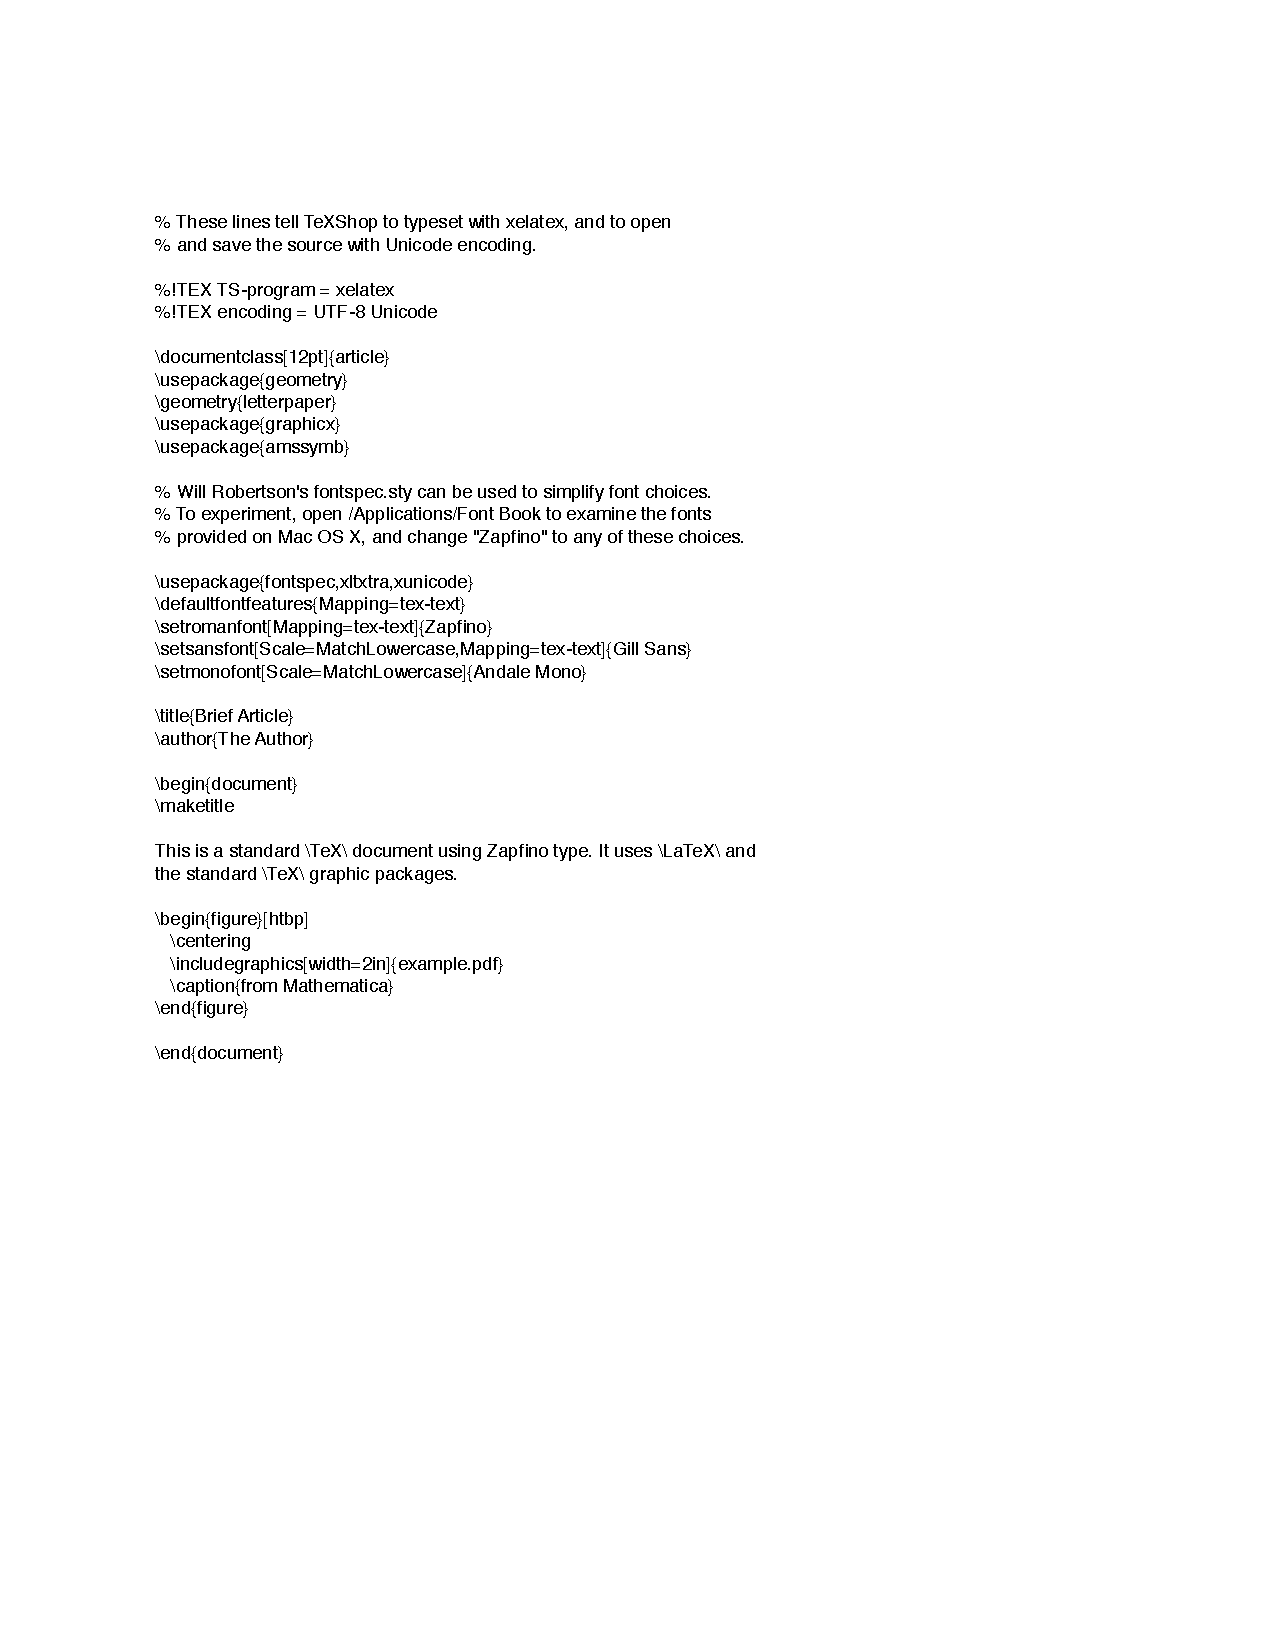
\includepdf{ZapfinoSourcePDF}

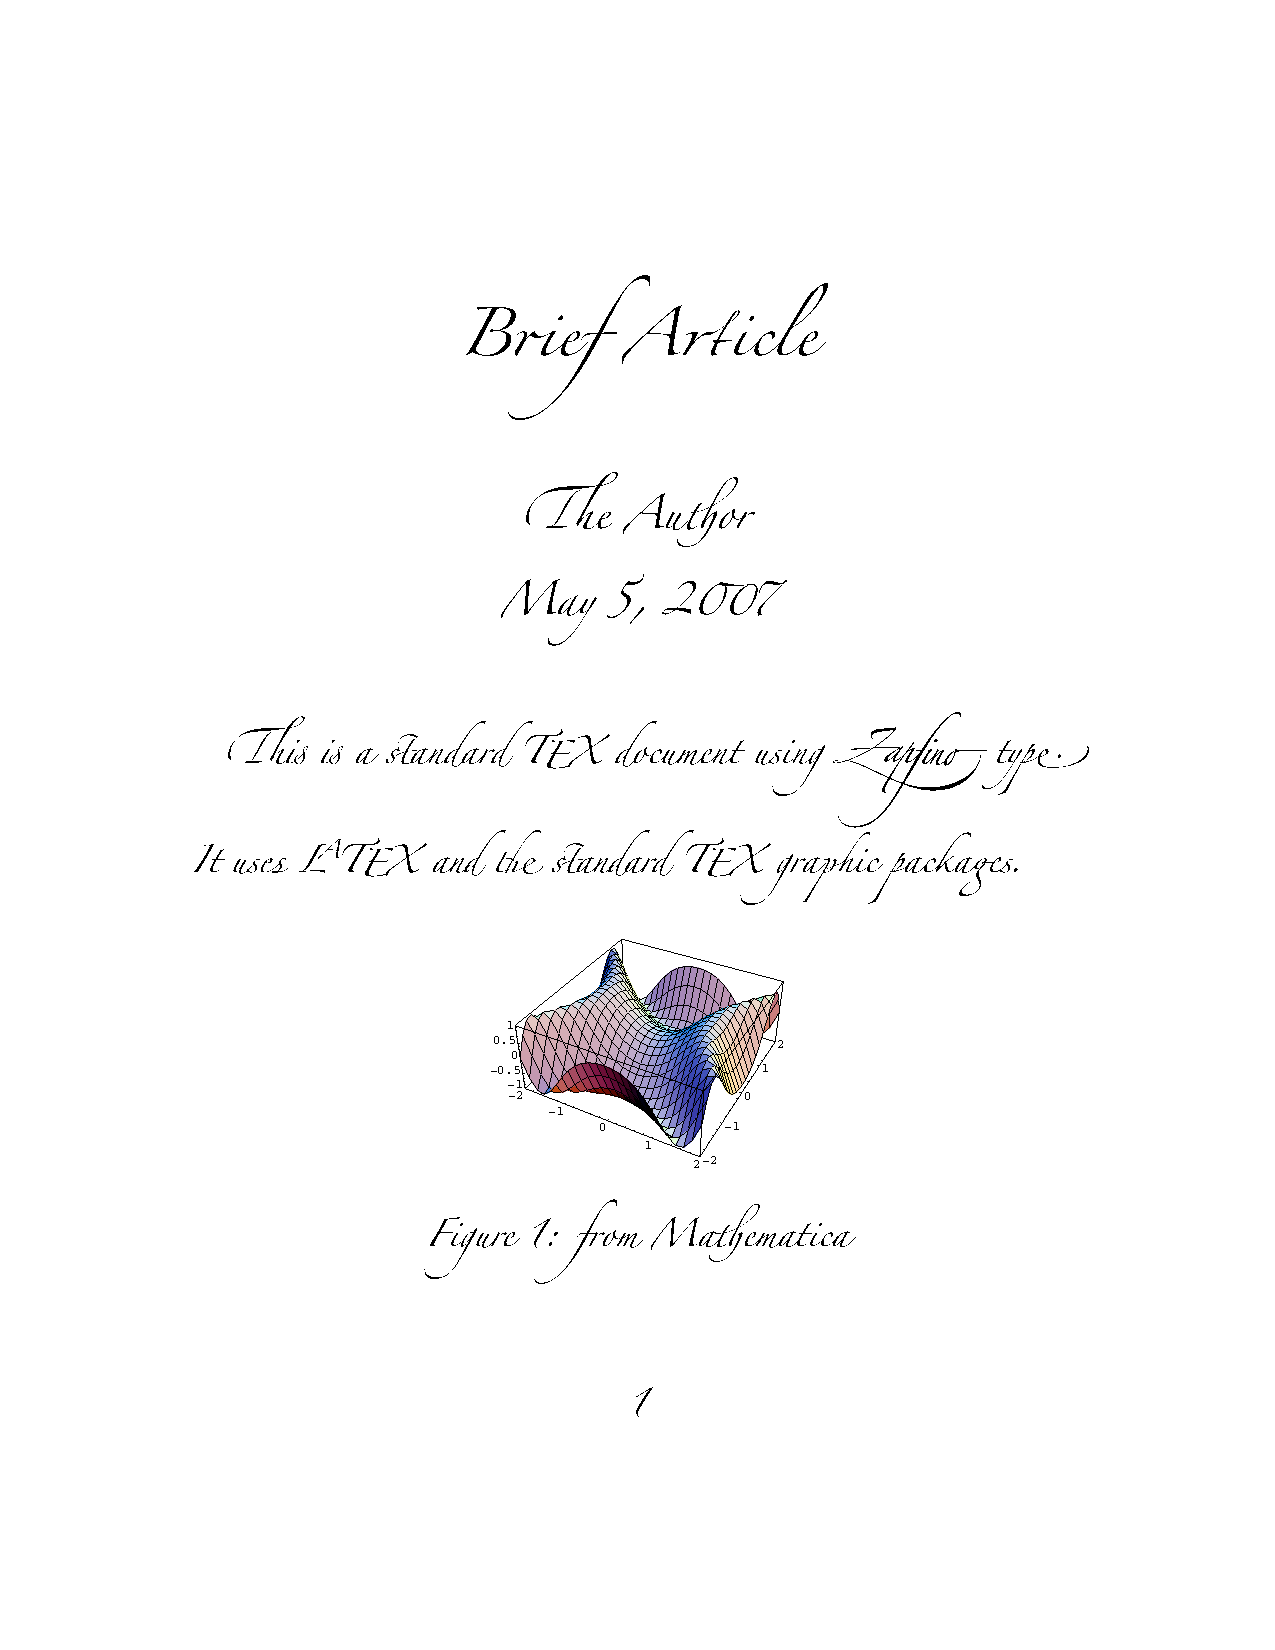
\includepdf{ZapfinoSource}

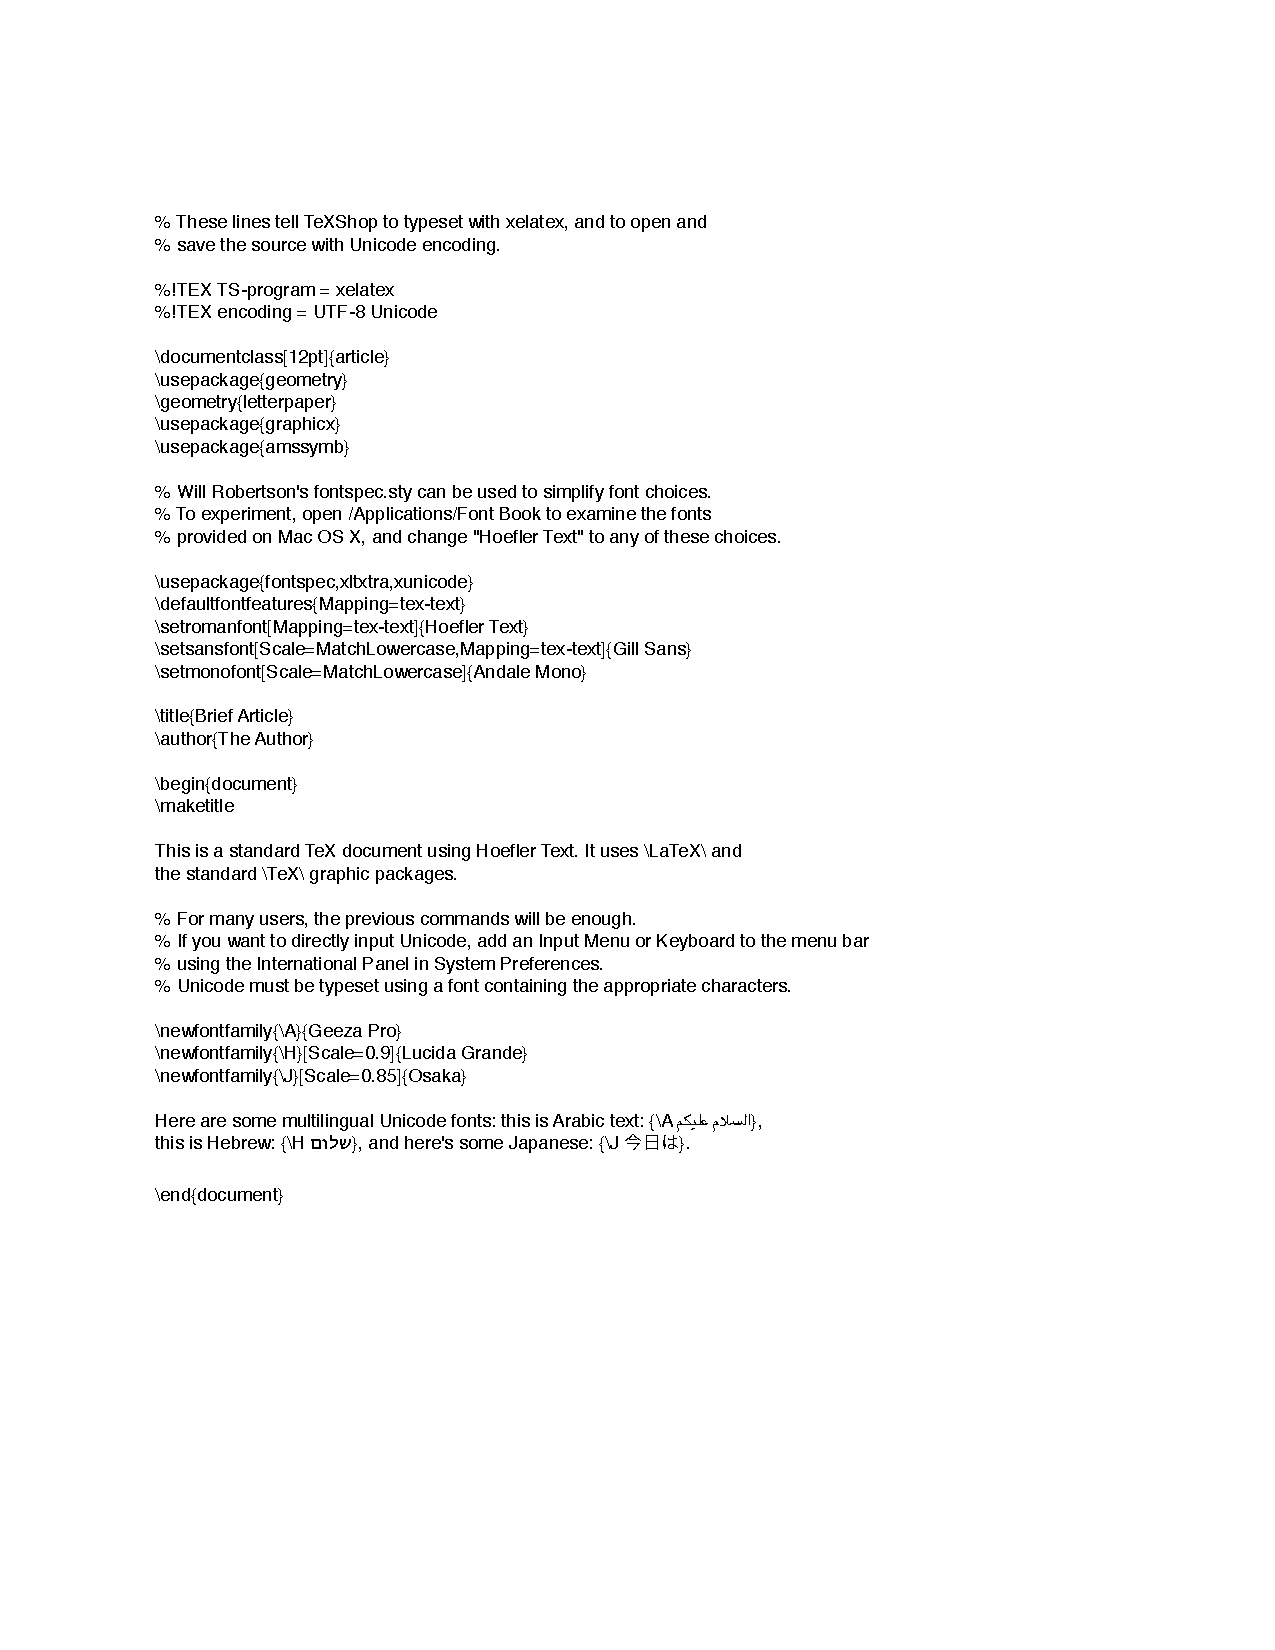
\includepdf{ScriptSourcePDF}

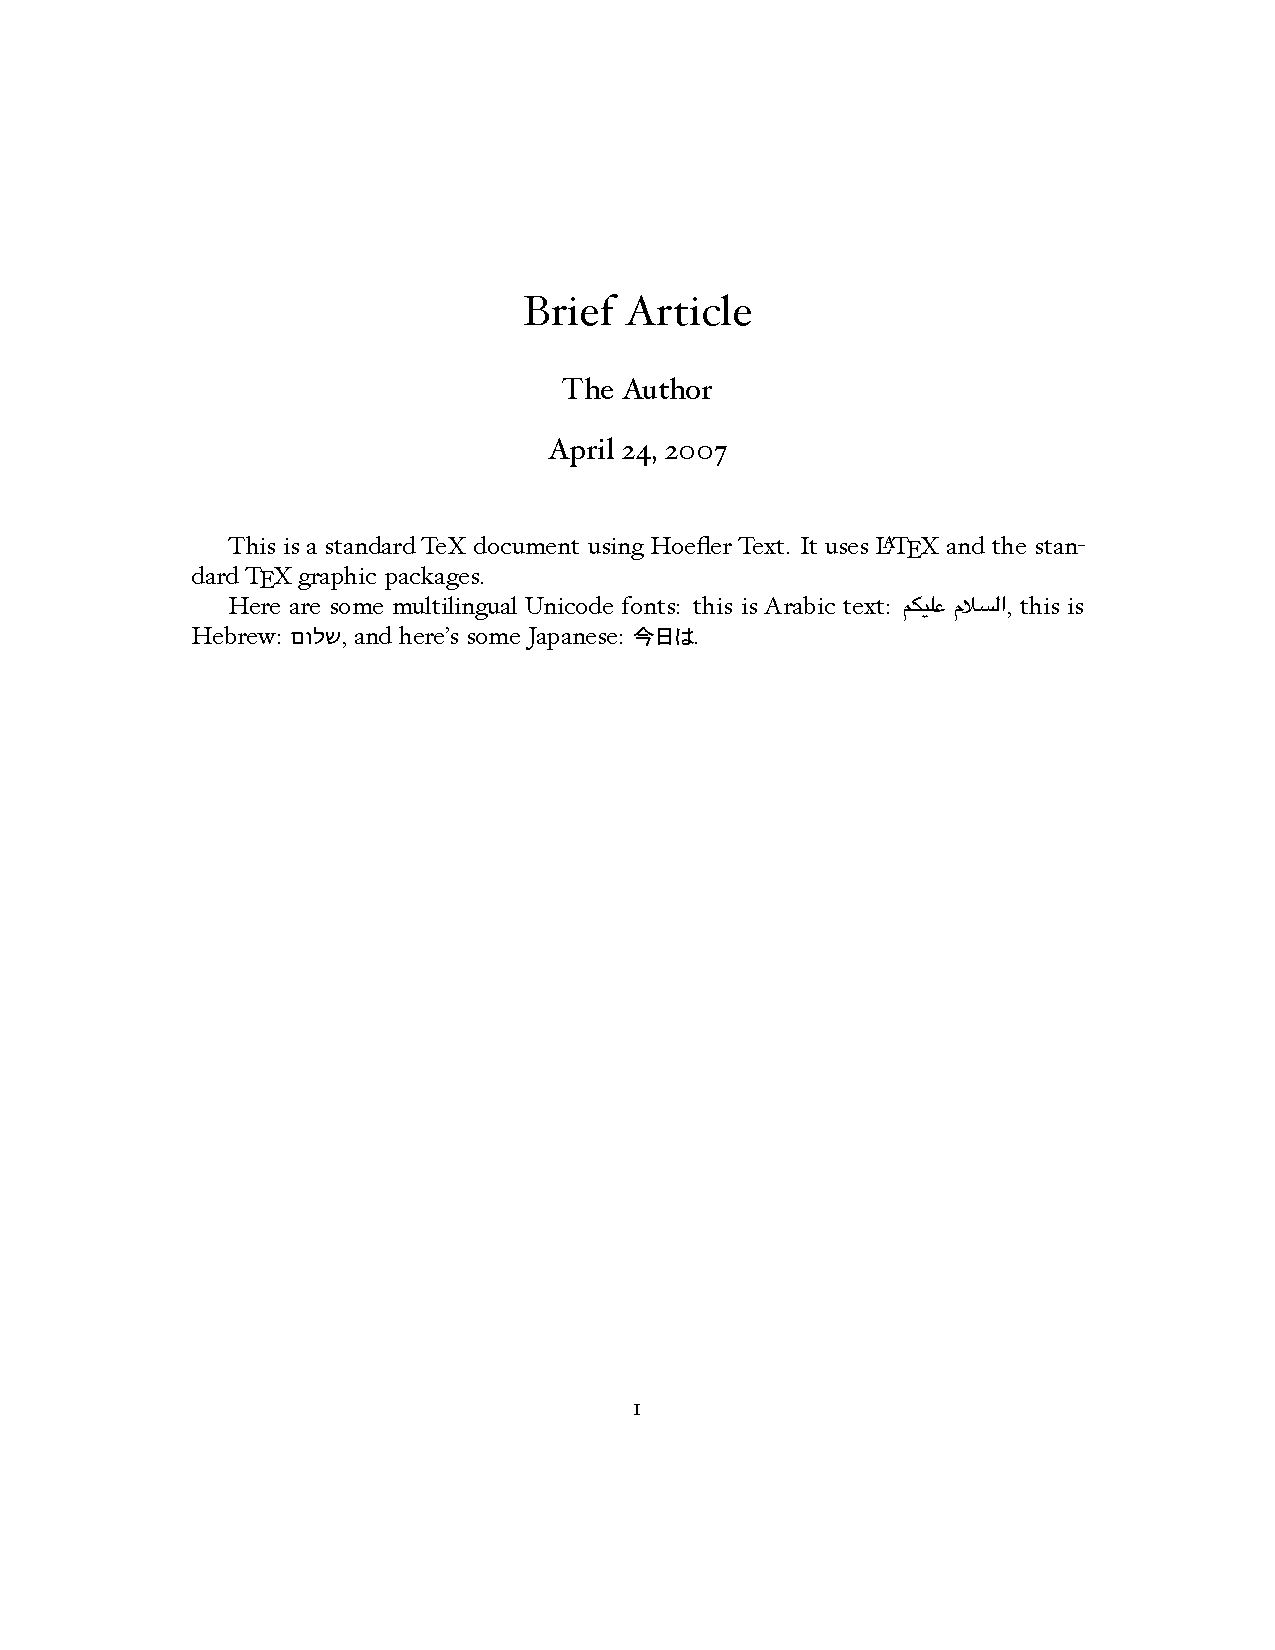
\includepdf{ScriptSource}



\end{document}  